\subsection{The relative kinematic}


We try to explain the difference between the microstructure configuration with an analysis of the averaged relative velocity fields $\textbf{w}^\text{nst}$. 
In this section we revisit the methodology used in \citet{zhang2023evolution} to describe the relative kinematic. 
That is to say that we give a quantitative description of the particles relative velocity in terms of the relative position and age of the interaction. 
Upon having a good estimation of this velocity field one is able to reconstruct the history of the particles interactions. 

% \end{figure}

\paragraph*{The impact of the Galileo number : }
The first effect that we present is the impact of the inertial effect on the particles relative kinematic. 
Here we investigate the impact of the inertial effect on the nature of the relative motion. 
As observed on \ref{fig:Pnst_high_Ga} and \ref{fig:Pnst_low_Ga} the impact of the Galileo seem greater for $\lambda=1$.
Therefore, we choose to expose the relative velocity fields for two cases : $Ga=10,100$ with $\lambda=1$, as the difference is more explicit. 
\begin{figure}[h!]
    \centering
    % \includegraphics[width=5cm]{image/HOMOGENEOUS_NEW/Dist/U_rel_l_10_Ga_10_PHI_5.pdf}
    \includegraphics[height=0.3\textwidth]{image/HOMOGENEOUS_NEW/Dist/U_rel_l_1_Ga_10_PHI_5.pdf}
    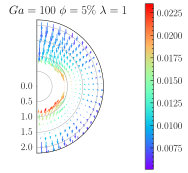
\includegraphics[height=0.3\textwidth]{image/HOMOGENEOUS_NEW/Dist/U_rel_l_1_Ga_100_PHI_5.pdf}
    % \includegraphics[width=5cm]{image/HOMOGENEOUS_NEW/Dist/U_rel_l_10_Ga_100_PHI_10.pdf}
    % \includegraphics[width=5cm]{image/HOMOGENEOUS_NEW/Dist/U_rel_l_1_Ga_100_PHI_10.pdf}
    \caption{Quiver plots of the relative averaged velocity field $\textbf{w}^\text{nst}(\textbf{r},a)$.
    The color map representing the age of the interaction, the early interaction are in dark blue for red for the long time interaction.
    (left) Low \textit{Galileo} number $Ga = 10$.
    (right) High \textit{Galileo} number $Ga = 25$. }
    \label{fig:Why_Ga_matter}
\end{figure}
From \ref{fig:Why_Ga_matter}  we remark that there is a clear asymmetry on the horizontal plan. 
Indeed, as a matter of fact the particles below the test sphere process all vertical velocity. 
One might expect a fore-after symmetry since we are studying pairs of particles. 
Then, how it is that the particle has nearest neighbors coming from the bottom than from the top ? 
First, one has to understand that $P_\text{nst}$ isn't a symmetric function due to the non commutativity of the function $h_{ij}$ in its definition, see \ref{eq:P_nstij}. 
Second, if the neighboring nearest particle is far from the test particle, the chance for this particle to have the test sphere as its nearest neighbor is low. 
Which means that in \ref{fig:Why_Ga_matter} we observe two distinct interaction from the test sphere with its nearest neighbors on the top and on the bottom. 
This disparity is due to the wake of generated by the test particle which tends to attract the particle at the bottom and to push those on the top. 

Following the color map and the vector fields, it can be stated that on average, the nearest neighboring particles approach from the vertical directions and leave
through the sides of the particle of reference. 
In fact, the fields $\textbf{w}^\text{nst}(r, a)$ provide a quantitative averaged representation of what is known as the \textit{Drafting Kissing Tumbling}\citep{fortes1987nonlinear} mechanism even if for $\lambda = 1$ other non-viscous effects may be important \citet{legendre2003hydrodynamic}.

Now let's investigate the disparity between the low and high inertial cases. 
As shown by \ref{fig:Why_Ga_matter} (left), at low \textit{Galileo} number the nearest particle has a tendency to get around the test particle.
Indeed, for high \textit{Galileo} number the relative velocity is nearly null on the sides and below the test particle, whereas for low \textit{Galileo} number the velocity has a clear non-null vertical component. 
Additionally, it is interesting to notice that,  at $\phi = 0.05$ the long interaction was situated on the sides of the test particle, while at $\phi = 0.1$ it is situated in the zone at below right from the test particle. 
The particles situated at the contact of the test particle results from early interaction. 
In brief for $Ga = 10$ it seems that the particle has no difficulty to get around the test particle on the sides, where for a $Ga = 100$ the relative velocity vanish in what seem to be a stagnation zone.


\paragraph*{The volume fraction dependency :}
As it has been observed in both \ref{fig:Pnst_high_Ga} and \ref{fig:Pnst_low_Ga} the effect of particle volume fraction is that it makes the particle distribution more concentrated on the sides of the test particle. 
\begin{figure}[h!]
    \centering
    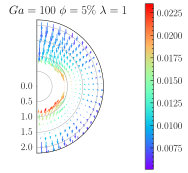
\includegraphics[width=5cm]{image/HOMOGENEOUS_NEW/Dist/U_rel_l_1_Ga_100_PHI_5.pdf}
    \includegraphics[width=5cm]{image/HOMOGENEOUS_NEW/Dist/U_rel_l_1_Ga_100_PHI_10.pdf}
    % \includegraphics[width=5cm]{image/HOMOGENEOUS_NEW/Dist/U_rel_l_10_Ga_100_PHI_10.pdf}
    % \includegraphics[width=5cm]{image/HOMOGENEOUS_NEW/Dist/U_rel_l_1_Ga_100_PHI_10.pdf}
    \caption{Quiver plots of the relative averaged velocity field $\textbf{w}^\text{nst}(\textbf{r},a)$.
    The color map representing the age of the interaction, the early interaction are in dark blue for red for the long time interaction.
    (left) Low \textit{Galileo} number $Ga = 10$.
    (right) High \textit{Galileo} number $Ga = 25$. }
    \label{fig:Why_Phi_matter}
\end{figure}
In \ref{fig:Why_Phi_matter} both graph exhibit the same stagnation zone where the particles result from a long interaction (dark red color) and the particle at contact from short interaction (dark blue color). 
The fact that the interaction at contact is early doesn't mean that the neighboring particles come quickly, it just means that they were already close. 
Additionally, the relative velocity have a high tendency to be oriented downward. 
Overall, the physical interaction doesn't seem to change in this range of volume fraciton. 

\paragraph*{The viscosity ratio dependency :}
Lastly, we now turn our attention to the effect of the viscosity ratio on pair interaction.
The question that we are trying to answer is : why does a smaller viscosity ratio increase the probability density on the horizontal plane ? 
The first point might be explained comparing 2 cases at $Ga = 100$ where we observe a clear difference between the PDF (see \ref{fig:Pnst_high_Ga}) for $\lambda = 1$ and  $\lambda = 10$.
\begin{figure}[h!]
    \centering
    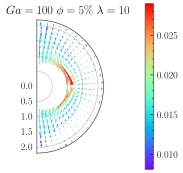
\includegraphics[width=5cm]{image/HOMOGENEOUS_NEW/Dist/U_rel_l_10_Ga_100_PHI_5.pdf}
    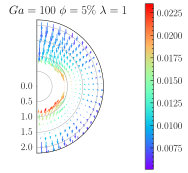
\includegraphics[width=5cm]{image/HOMOGENEOUS_NEW/Dist/U_rel_l_1_Ga_100_PHI_5.pdf}
    % \includegraphics[width=5cm]{image/HOMOGENEOUS_NEW/Dist/F_rel_l_10_Ga_100_PHI_5.pdf}
    % \includegraphics[width=5cm]{image/HOMOGENEOUS_NEW/Dist/F_rel_l_1_Ga_100_PHI_5.pdf}
    \caption{Quiver plots of the relative averaged velocity field $\textbf{w}^\text{nst}(\textbf{r},a)$.
    The color map representing the age of the interaction, the early interaction are in dark blue for red for the long time interaction.
    (left) High viscosity ratio $\lambda = 10$, solid-like particle.
    (right) Low viscosity ratio, $\lambda = 1$ bubble-like particle. }
    \label{fig:Why_l_matter}
\end{figure}
The age is represented by the color map from dark blue for earliest interaction to dark red for the longest interaction. 
To track the course of the averaged path of the nearest particle one has to follow the flow lines $\textbf{w}^\text{nst}$. 
It is then clear from \ref{fig:Why_l_matter} (left) and (right) that the neighboring particle approach on the vertical direction and end up its course on the sides. 
Therefore, it explains why the particles' concentration tends to be higher on the sides as seen in \ref{fig:Pnst_high_Ga}. 
At low $\lambda$ it is seen in \ref{fig:Why_l_matter} (right) that the particle reaches a quasi null relative velocity on the sides. 
Indeed, we identify a clear stagnation zone where the age is maximum and the relative velocity is nearly null. 
On the other hand for $\lambda =10$ the relative velocity on the vicinity of the particle of reference isn't as much as low as for the previous case.
Additionally,  the particles reaches their maximum age while being in contact of the test particle.
This testifies to the interruption of the interaction by another particle. 
Indeed, if the particle in contact of the test sphere suddenly stop being the nearest particle it means that its has been replaced by an other particle. 
In brief, for $\lambda =1$ the particle seem to have lost all of its relative momentum at the end of the interaction leaving them side by side, while when $\lambda =10$ the neighboring particle is still in motion.  
At lower $Ga$ we observe no difference between the velocity fields of two different viscosity ratios. 
At higher volume fraction same comments than above can be made. 
This is consistent with the PDF displayed in \ref{fig:Pnst_low_Ga} where we observed no changes with $\lambda$. 

Overall :
\begin{itemize}
    \item The impact of Galileo is that long interaction arise far from the particle and with no relative velocity, while at low $Ga$ the long interaction can happen on the side.
    \item The volume fraction impact is that long interaction are even further away from the particle. 
    \item The viscosity ratio change the nature of the interaction by rapproching the rad zone. 
    It does mean that there is more close contact long interaction type.
\end{itemize}

The ability of the neighboring particle to stay close to the test particle seems to be the keys to fin out the main difference in behavior between the $\lambda=1$ and  $\lambda = 10$ cases. 
Indeed, as a matter of fact partcile 

\tb{Compare the velocity with \citet{shajahan2023inertial}}

\tb{The asymmetry of the velocity come form the layers in which case bubbles that comming from botton etc is different}